\documentclass[crop,tikz]{standalone}
\usetikzlibrary{calc}
\usetikzlibrary{arrows}
\usetikzlibrary{decorations.pathreplacing}
\begin{document}
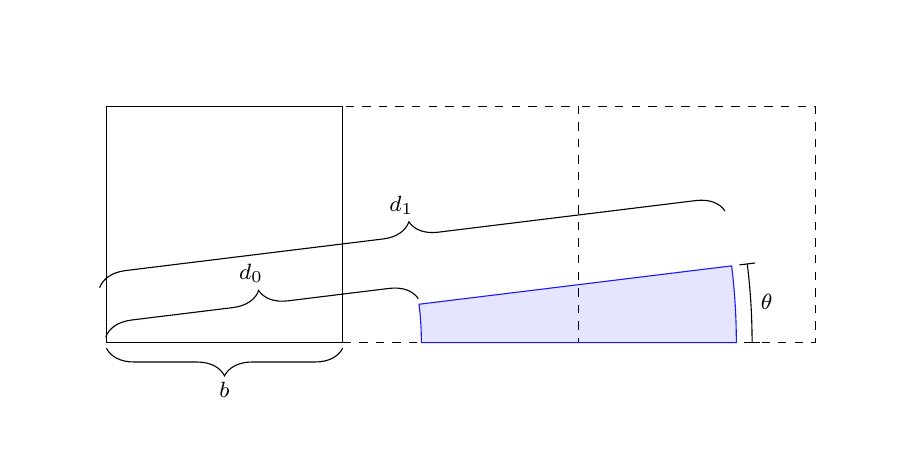
\begin{tikzpicture}
  % Constants
  \pgfmathsetmacro\b{3}
  \pgfmathsetmacro\d{8}
  \pgfmathsetmacro\c{4}
  \pgfmathsetmacro\t{7}
  \pgfmathsetmacro\a{0}
  % Boundary
  \path[use as bounding box] (0,0) rectangle (2+\b*3,2+\b);
  % Domain grids
  \draw (1,1) -- (1+\b,1) -- (1+\b,1+\b) -- (1,1+\b) -- cycle;
  \draw[dashed] (1+\b,1) -- (1+2*\b,1) -- (1+2*\b,1+\b) -- (1+\b,1+\b);
  \draw[dashed] (1+2*\b,1) -- (1+3*\b,1) -- (1+3*\b,1+\b) -- (1+2*\b,1+\b);
  % Domain size
  \draw[decorate,decoration={brace,mirror,amplitude=10pt},yshift=-2] (1,1) -- (1+\b,1) node [midway,yshift=-15] {\footnotesize $b$};
  % Lightcone
  \begin{scope}[shift={(1,1)}]
    \filldraw[fill=blue,fill opacity=0.1,draw=blue!90] (\a:\c) arc (\a:\a+\t:\c) -- (\a+\t:\d) arc (\a+\t:\a:\d) -- cycle;
    % Theta
    \draw (\a:\d+0.1) -- (\a:\d+0.3);
    \draw (\a+\t:\d+0.1) -- (\a+\t:\d+0.3);
    \draw (\a:\d+0.2) arc (\a:\a+\t:\d+0.2);
    \node at (\a+\t/2:\d+0.4) {\footnotesize $\theta$};
    % Length of c and d
    \draw[decorate,decoration={brace,amplitude=10pt},rotate=\a+\t,yshift=20] (0,0) -- (\d,0) node [midway,xshift=-4,yshift=16] {\footnotesize $d_1$};
    \draw[decorate,decoration={brace,amplitude=10pt},rotate=\a+\t,yshift=2] (0,0) -- (\c,0) node [midway,xshift=-4,yshift=16] {\footnotesize $d_0$};
  \end{scope}
\end{tikzpicture}
\end{document}
